\documentclass[12pt]{article}
\usepackage{scrextend}
\usepackage[utf8]{inputenc}
\usepackage[polish]{babel}
\usepackage[T1]{fontenc}%polskie znaki
\usepackage[utf8]{inputenc}%polskie znaki
\usepackage{geometry}
\usepackage{float}
\usepackage{enumitem}
\usepackage{hyperref}
\usepackage{graphicx}
\usepackage{tabulary}
\usepackage{etoc}
\usepackage[normalem]{ulem} 
\renewcommand{\baselinestretch}{1.5}
\graphicspath{ {img/} }
\newgeometry{lmargin=2.0cm, rmargin=2.0cm, tmargin=2.0cm, bmargin=2.0cm}
\usepackage{tikz}
\usepackage[bf]{caption}
\usepackage{dirtytalk}
\usepackage{listings}
\usepackage{xcolor}
\newcommand{\paragraphnewline}[1]{\paragraph{#1}\mbox{}\\}



\definecolor{codegreen}{rgb}{0,0.6,0}
\definecolor{codegray}{rgb}{0.5,0.5,0.5}
\definecolor{codepurple}{rgb}{0.58,0,0.82}
\definecolor{backcolour}{rgb}{0.95,0.95,0.92}

\lstdefinestyle{mystyle}{
    backgroundcolor=\color{backcolour},   
    commentstyle=\color{codegreen},
    keywordstyle=\color{magenta},
    numberstyle=\tiny\color{codegray},
    stringstyle=\color{codepurple},
    basicstyle=\ttfamily\footnotesize,
    breakatwhitespace=false,         
    breaklines=true,                 
    captionpos=b,                    
    keepspaces=true,                 
    numbers=left,                    
    numbersep=5pt,                  
    showspaces=false,                
    showstringspaces=false,
    showtabs=false,                  
    tabsize=2
}

\title{ 
    \vspace*{50mm}
    \textsc{
        \textbf{Rozpoznawanie i Przetwarzanie Obrazów}\\
        \large Generator masek real-time \\
        \normalsize Zadanie 2 - Opis programu 
    }
} 
\author{
Maja Bojarska, 241287\\
Wiktor Pieklik, 241282\\
Grupa projektowa nr 2\\
}

\date{\today}

\begin{document}

\maketitle

% \setcounter{tocdepth}{2}
% \localtableofcontents
% \listoffigures
% \lstlistoflistings

\clearpage
\section{Wymagania}
\subsection{Funkcjonalne}
Jako użytkownik:
\begin{itemize}
    \item chcę nakładać maskę na obraz przechwytywany przez kamerę w czasie rzeczywistym,
    \item chcę móc wybrać konkretną maskę, spośród listy oferowanych masek,
    \item chcę móc zrobić zdjęcie, aby je zapisać na dysku,
    \item chcę móc nagrać film, aby go zapisać na dysku
\end{itemize}
\subsection{Niefunkcjonalne}
\begin{itemize}
    \item Aplikacja działa jako aplikacja desktopowa,
    \item aplikacja zrównolegla pobieranie klatek z kamery i ich przetwarzanie,
    \item aplikacja nie potrzebuje dostępu do internetu w trakcie swojego działania
\end{itemize}

\subsection{Aplikacja}
\subsubsection{View}
\begin{itemize}
    \item Posiada okno z podglądem obrazu,
    \item oferuje wybór jeden spośród wielu masek,
    \item przycisk \say{włącz/wyłącz maskę},
    \item przycisk \say{Zrób zdjęcie},
    \item przycisk \say{Uruchom/zatrzymaj nagrywanie},
    \item opcjonalne wyświetlanie wykrytych punktów charakterystycznych twarzy.
\end{itemize}
\subsubsection{Controller}
\begin{itemize}
    \item Posiada osobny wątek/proces przetwarzający ramki za pomocą ImageProcessor,
    \item Posiada osobny wątek/proces przechwytujący ramki za pomocą instancji klasy VideoSource
\end{itemize}

\subsection{Przykłady masek nakładanych real-time}
\subsubsection{Nakładana grafika}
\begin{itemize}
    \item Okulary,
    \item wąsy,
    \item fryzura.
\end{itemize}
\subsubsection{Przekształcenia geometrii}
\begin{itemize}
    \item Powiększanie oczu/ust
\end{itemize}

\clearpage
\section{Architektura systemu}

\begin{figure}[H]
    \centering
    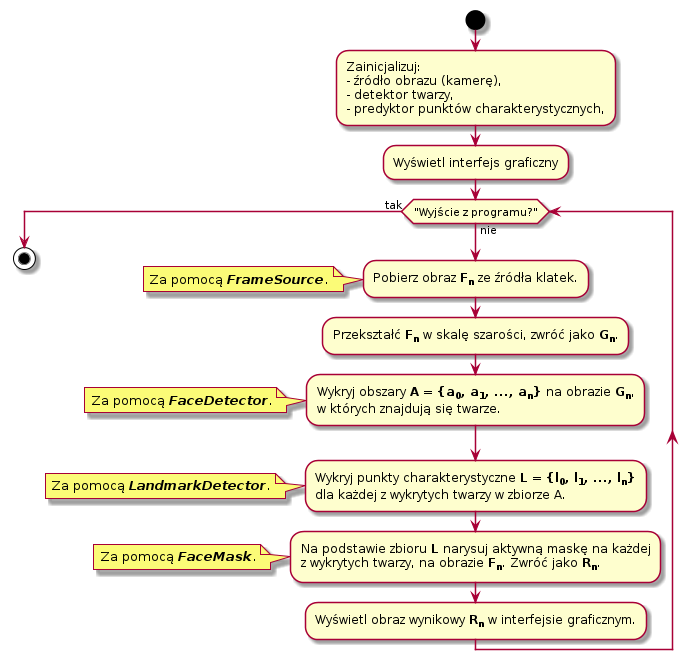
\includegraphics[width=\linewidth]{diagrams/out/data_flow.png}
    \caption{}
    \label{}
\end{figure}

\end{document}
